\documentclass[oneside,12pt,letterpaper]{article}

% Imports and Definitions
%% Packages
\usepackage{amsmath}
\usepackage{amsfonts}
\usepackage{amssymb}
\usepackage{amsthm}
\usepackage{arydshln}
\usepackage{color}
\usepackage{extramarks}
\usepackage{fancyhdr}
\usepackage{float}
\usepackage[margin=1in]{geometry}
\usepackage{graphicx}
\usepackage{listings}
\usepackage{multicol}
\usepackage{setspace}
\usepackage{subcaption}
\usepackage{textcomp}
\usepackage{url}
\usepackage{xspace}
\usepackage{mathtools}

%% Commands
%%% Metadata
\newcommand{\metaTitle}{Comprehensive Exam}
\newcommand{\metaDueDate}{November 24, 2020}
\newcommand{\metaDueTime}{04:00 PM}
\newcommand{\metaSchool}{IUPUI}
\newcommand{\metaClass}{STAT 52400}
\newcommand{\metaDepartment}{Statistics Department}
\newcommand{\metaAuthorName}{Ross Grinvalds}

%%% Aliases
\newcommand{\Bias}{\mathrm{Bias}}
\newcommand{\Cov}{\mathrm{Cov}}
\newcommand{\dd}[1]{\frac{\mathrm{d}}{\mathrm{d}x} (#1)}
\newcommand{\dx}{\mathrm{d}x}
\newcommand{\E}{\mathrm{E}}
\newcommand{\m}[1]{\begin{bmatrix*}[r]#1\end{bmatrix*}}
\newcommand{\md}[1]{\begin{vmatrix*}#1\end{vmatrix*}}
\newcommand{\mf}[1]{\mathrm{\bf{#1}}}
\newcommand{\p}[1]{\begin{pmatrix}#1\end{pmatrix}} 
\newcommand{\pdd}[2]{\frac{\partial}{\partial #1} (#2)}
\newcommand{\solution}{\textbf{\large Solution}}
\newcommand{\T}{\intercal}
\newcommand{\Var}{\mathrm{Var}}

%%% Math Functions
\makeatletter
\newsavebox{\mybox}\newsavebox{\mysim}
\newcommand{\distras}[1]{%
  \savebox{\mybox}{\hbox{\kern3pt$\scriptstyle#1$\kern3pt}}%
  \savebox{\mysim}{\hbox{$\sim$}}%
  \mathbin{\overset{#1}{\kern\z@\resizebox{\wd\mybox}{\ht\mysim}{$\sim$}}}%
}
\makeatother

\newcommand{\indep}{\perp \!\!\! \perp}

%% Environments
%%% R Code
\newcommand{\ri}[1]{\lstinline{#1}}  %% Short for 'R inline'

\lstnewenvironment{rc}[1][]{
	\lstset{commentstyle=\color{red}, keywordstyle=\color{black}, showstringspaces=true, language=R, basicstyle=\ttfamily\tiny}
}{}
\lstset{language=R}


% Settings
%% Document-wide
\pagestyle{fancy}

%% Header and Footer
\setlength{\headheight}{15pt}
\lhead{\metaAuthorName}
\chead{\metaSchool\ \metaClass:\ \metaTitle}
\rhead{\metaDepartment}
\cfoot{\thepage}

%% Title Page
\title{
	\vspace{1in}
	\textmd{\textbf{\metaSchool\ \metaClass:\ \metaTitle}}\\
	\normalsize\vspace{0.1in}\small{Due\ by\ \metaDueDate\ at \metaDueTime}\\
	\vspace{6in}
}
\author{\metaAuthorName}
\date{}


\begin{document}
\maketitle

\section*{Problem 8.20} 
\begin{enumerate}
\item[\bf{a)}]
	National track record data in Table 8.6 is considered for this analysis. Each of the columns of this data set represents a different track event, ordered from shortest to longest event. The correlation matrix, $\mf{R}$, is given below, along with the eigenvalues and eigenvectors.

\begin{rc}

> R
          X2        X3        X4        X5        X6        X7        X8        X9
X2 1.0000000 0.9147554 0.8041147 0.7119388 0.7657919 0.7398803 0.7147921 0.6764873
X3 0.9147554 1.0000000 0.8449159 0.7969162 0.7950871 0.7613028 0.7479519 0.7211157
X4 0.8041147 0.8449159 1.0000000 0.7677488 0.7715522 0.7796929 0.7657481 0.7126823
X5 0.7119388 0.7969162 0.7677488 1.0000000 0.8957609 0.8606959 0.8431074 0.8069657
X6 0.7657919 0.7950871 0.7715522 0.8957609 1.0000000 0.9165224 0.9013380 0.8777788
X7 0.7398803 0.7613028 0.7796929 0.8606959 0.9165224 1.0000000 0.9882324 0.9441466
X8 0.7147921 0.7479519 0.7657481 0.8431074 0.9013380 0.9882324 1.0000000 0.9541630
X9 0.6764873 0.7211157 0.7126823 0.8069657 0.8777788 0.9441466 0.9541630 1.0000000

> eigen(R)
eigen() decomposition
\$values
[1] 6.703289951 0.638410110 0.227524494 0.205849181 0.097577441 0.070687912 0.046942050 0.009718862

\$vectors
           [,1]        [,2]         [,3]        [,4]        [,5]        [,6]       [,7]         [,8]
[1,] -0.3323877 -0.52939911 -0.343859303  0.38074525  0.29967117 -0.36203713  0.3476470 -0.065701445
[2,] -0.3460511 -0.47039050  0.003786104  0.21702322 -0.54143422  0.34859224 -0.4398969  0.060755403
[3,] -0.3391240 -0.34532929  0.067060507 -0.85129980  0.13298631  0.07708385  0.1135553 -0.003469726
[4,] -0.3530134  0.08945523  0.782711152  0.13427911 -0.22728254 -0.34130845  0.2588830 -0.039274027
[5,] -0.3659849  0.15365241  0.244270040  0.23302034  0.65162403  0.52977961 -0.1470362 -0.039745509
[6,] -0.3698204  0.29475985 -0.182863147 -0.05462441  0.07181636 -0.35914382 -0.3283202  0.705684585
[7,] -0.3659489  0.33360619 -0.243980694 -0.08706927 -0.06133263 -0.27308617 -0.3511133 -0.697181715
[8,] -0.3542779  0.38656085 -0.334632969  0.01812115 -0.33789097  0.37516986  0.5941571  0.069316891
\end{rc}

\item[\bf{b)}]
	Next, the standardized variables were obtained and a principal component analysis was performed on the data. The eigenvalues and eigenvectors of the correlation matrix are provided below. Given the large magnitude of the first eigenvalue, the first principal component appears to explain a large portion of the variation in the data.

\begin{rc}

> eigen(Rz)
eigen() decomposition
\$values
[1] 6.703289951 0.638410110 0.227524494 0.205849181 0.097577441 0.070687912 0.046942050 0.009718862

\$vectors
           [,1]        [,2]         [,3]        [,4]        [,5]        [,6]       [,7]         [,8]
[1,] -0.3323877 -0.52939911  0.343859303  0.38074525 -0.29967117 -0.36203713  0.3476470 -0.065701445
[2,] -0.3460511 -0.47039050 -0.003786104  0.21702322  0.54143422  0.34859224 -0.4398969  0.060755403
[3,] -0.3391240 -0.34532929 -0.067060507 -0.85129980 -0.13298631  0.07708385  0.1135553 -0.003469726
[4,] -0.3530134  0.08945523 -0.782711152  0.13427911  0.22728254 -0.34130845  0.2588830 -0.039274027
[5,] -0.3659849  0.15365241 -0.244270040  0.23302034 -0.65162403  0.52977961 -0.1470362 -0.039745509
[6,] -0.3698204  0.29475985  0.182863147 -0.05462441 -0.07181636 -0.35914382 -0.3283202  0.705684585
[7,] -0.3659489  0.33360619  0.243980694 -0.08706927  0.06133263 -0.27308617 -0.3511133 -0.697181715
[8,] -0.3542779  0.38656085  0.334632969  0.01812115  0.33789097  0.37516986  0.5941571  0.069316891
\end{rc}

The correlation of the standardized variables with the components for the first two principal components is given along with the eigenvalues and the total proportion of explained variance. The first two principal components account for $91.7\%$ of the variation in the data. The magnitudes of the correlations help to identify which of the variables demonstrate the strongest impact on the associated principal component. For the first principal component, all of the variables have a similar magnitude, suggesting that they all offer an equal impact. For the second, both the 800 meter and 1500 meter events have a smaller magnitude than the rest of the variables. This makes sense given the interpretation that follows in part $\bf{c}$. 

\begin{rc}

> table
        rho_Y1X     rho_Y2X  eigenvalue proportion
[1,] -0.8605755 -0.42299290 6.703289951  0.8379112
[2,] -0.8959509 -0.37584469 0.638410110  0.9177125
[3,] -0.8780162 -0.27592007 0.227524494  0.9461531
[4,] -0.9139768  0.07147524 0.205849181  0.9718842
[5,] -0.9475610  0.12276915 0.097577441  0.9840814
[6,] -0.9574913  0.23551480 0.070687912  0.9929174
[7,] -0.9474679  0.26655325 0.046942050  0.9987851
[8,] -0.9172508  0.30886432 0.009718862  1.0000000
\end{rc}


\item[\bf{c)}]
	The first principal component seems to suggest that each of the track event categories contributes roughly equally to the variance in the data set. Because each of these events is hosted separately from the others, and because there are world class athletes competing in each of the events, this naturally makes sense. The second principal component suggests that there is an inverse correspondence between events that have short distances (100, 200, and 400 meters) and events that have long distances (greater than 400 meters). Considered together, the first component helps to provide a weight to each of the events, and the second component contrasts short and long events.

\item[\bf{d)}]
	A ranking of men's track events by nation based on the first principal component is provided below. It does correspond to my own assumptions about what nations ought to have performed well in track events.

\begin{rc}

 [1,] "U.S.A."         "3.82842499343348"   
 [2,] "GreatBritain"   "2.91498277358019"   
 [3,] "Kenya"          "2.60834728893362"   

...

[52,] "Singapore"      "-3.6914922877556"   
[53,] "Samoa"          "-8.42153734747028"  
[54,] "CookIslands"    "-10.7111965079781"
\end{rc}

\item[\bf{e)}]
	The results for the women's track data are highly similar to the men's data. See selected output from the analysis below.

\begin{rc}

> table
        rho_Y1X    rho_Y2X eigenvalue proportion
[1,] -0.9103780 -0.3228503 5.80762446  0.8296606
[2,] -0.9234990 -0.3279673 0.62869342  0.9194740
[3,] -0.8869307 -0.3642220 0.27933457  0.9593789
[4,] -0.9513832  0.1278522 0.12455472  0.9771725
[5,] -0.9380805  0.2450762 0.09097174  0.9901684
[6,] -0.9063506  0.3355481 0.05451882  0.9979568
[7,] -0.8560043  0.3086096 0.01430226  1.0000000

 [1,] "USA"  "3.29914882340426"    
 [2,] "GER"  "3.04751660310563"    
 [3,] "RUS"  "3.04294821407376"   

...

[52,] "PNG"  "-5.25744974658153"   
[53,] "COK"  "-7.90622722445813"   
[54,] "SAM"  "-8.21341512287609"
\end{rc}

\end{enumerate}


\newpage
\section*{Problem 8.21} 
The men's track data used in problem $\bf{8.20}$ represents data from a variety of different track events. The event distances range from $100$ meters to a marathon's length. The shorter distance events are measured in seconds while the longer events are measured in minutes. This may pose a problem for a principal component analysis because the scale of the measurements distorts the comparative performance across events. A correction for this issue is to first standardize the variables to the same measurement. For the purpose of this analysis, first the data is converted to speed in meters per second for all of the recorded events.

\begin{rc}

> df.speeds
# A tibble: 54 x 9
   nation    `100m` `200m` `400m` `800m` `1.5km` `5km` `10k` marathon
   <chr>      <dbl>  <dbl>  <dbl>  <dbl>   <dbl> <dbl> <dbl>    <dbl>
 1 Argentina   9.78   9.82   8.66   7.53    6.79  6.25  6.03     5.43
 2 Australia  10.1    9.97   9.01   7.66    7.08  6.44  6.05     5.52
 3 Austria     9.85   9.78   8.73   7.53    6.98  6.28  6.01     5.32
 4 Belgium     9.86   9.91   8.88   7.71    7.00  6.50  6.20     5.53
 5 Bermuda     9.74   9.85   8.84   7.45    6.76  5.69  5.47     4.80
 6 Brazil     10     10.1    9.03   7.84    7.00  6.18  5.92     5.58
 7 Canada     10.2    9.92   8.94   7.62    7.08  6.30  6.04     5.41
 8 Chile       9.90   9.93   8.71   7.58    6.85  6.22  5.93     5.32
 9 China       9.83   9.79   8.84   7.53    6.93  6.21  5.92     5.44
10 Columbia    9.72   9.59   8.73   7.41    6.72  6.18  5.98     5.36
# ... with 44 more rows
\end{rc}

Next, an analysis similar to $\bf{8.20}$ is repeated on the data expressed in speed. This time, instead of using the correlation matrix, $\bf{R}$, the variance-covariance matrix, $\bf{S}$, is used. The proportion of variance explained by the first two variables is similar to $\bf{8.20}$ with a slight increase in the variance captured. The interpretation of the first two principal components is also the same. That is, the first component gives roughly equal importance to each of the track events, and the second component provides a contrast between shorter and longer events. The analysis using the data expressed as speed should be preferred to the original analysis, as it provides a more reasonable comparison for the performance across events.

\begin{rc}

> table
        rho_Y1X      rho_Y2X  eigenvalue proportion
[1,] -0.1714834 -0.092958577 0.494049954  0.8443571
[2,] -0.2188668 -0.112541618 0.046223803  0.9233560
[3,] -0.2226852 -0.100846223 0.013912284  0.9471328
[4,] -0.1950545 -0.007052284 0.013320803  0.9698987
[5,] -0.2560350  0.013511229 0.007522548  0.9827552
[6,] -0.3006149  0.056188829 0.005749212  0.9925809
[7,] -0.2958577  0.066624655 0.003220375  0.9980846
[8,] -0.2926614  0.083178195 0.001120710  1.0000000

 [1,] "U.S.A."         "-21.1082018492229"
 [2,] "Kenya"          "-20.9311588666277"
 [3,] "GreatBritain"   "-20.8500614768412"

 ...

[52,] "PapuaNewGuinea" "-18.9629795445273"
[53,] "Samoa"          "-17.849219213"    
[54,] "CookIslands"    "-17.3440198817945"
\end{rc}


\newpage
\section*{Problem 8.22}
\begin{enumerate}
\item[\bf{a)}]
	The data presented in Table $1.10$ represents the auction price and a selection of body measurements of young bulls. A principal component analysis of the body measurements for the sample variance-covariance matrix as well as the correlation matrix is desired. Beginning with the sample variance-covariance matrix, $\mf{S}$, it is clear that the first two principle components account for a dominant portion of the sample variation. This is also captured in the scree plot shown below on the left.

\begin{rc}

       eigenvalue total_proportion
[1,] 2.057961e+04        0.8081979
[2,] 4.874675e+03        0.9996351
[3,] 5.429170e+00        0.9998483
[4,] 3.316308e+00        0.9999785
[5,] 4.688301e-01        0.9999969
[6,] 7.405369e-02        0.9999998
[7,] 4.519442e-03        1.0000000
\end{rc}

	A principal component analysis of the correlation matrix, $\mf{R}$, provides a different interpretation. Analyzing the total proportion of variation explained by the principal components, this new analysis suggests that at least three of the components should be retained to adequately characterize the sample variation. The scree plot of this analysis suggests that two components may be suitable, however, a large portion of the sample variation will be dismissed if only two are selected.

\begin{rc}

     eigenvalue total_proportion
[1,]  4.1206979        0.5886711
[2,]  1.3371293        0.7796896
[3,]  0.7413825        0.8856014
[4,]  0.4214252        0.9458050
[5,]  0.1858059        0.9723487
[6,]  0.1465024        0.9932776
[7,]  0.0470567        1.0000000
\end{rc}

\begin{center}
	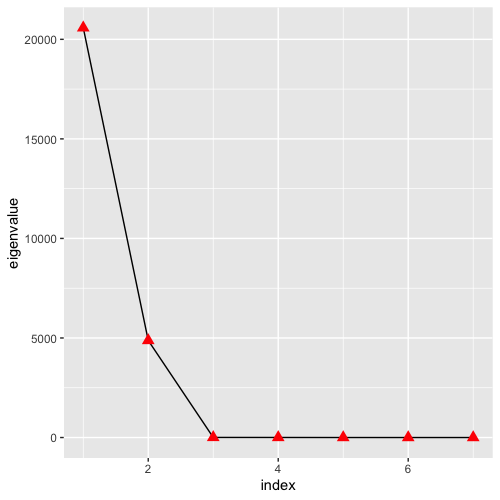
\includegraphics[width=3.0in]{8_22_S_scree.png}
	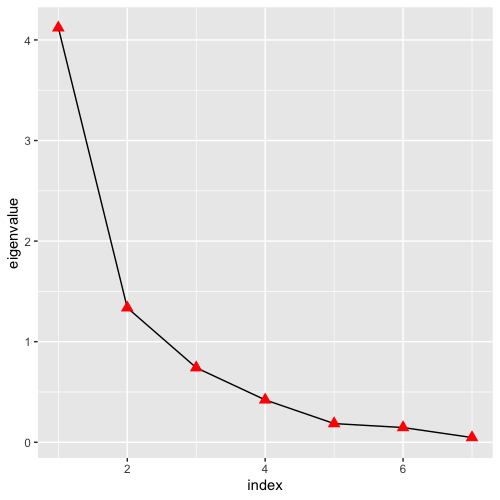
\includegraphics[width=3.0in]{8_22_R_scree.png}
\end{center}

\item[\bf{b-c)}]
	The results for the PCA on $\mf{S}$ suggest that the first two principal components will effectively summarize the variation contained in the sample. Analyzing the two corresponding eigenvectors along with the variable names allows for an interpretation of the principal components. The dominant variables in the first principal component are ``FtFrBody'' and ``SaleWt''. From the metadata, ``FtFrBody'' represents the fat free weight (pounds) of the bull. ``SaleWt'' represents the weight (pounds) of the bull upon sale. This suggests that the first principal component provides an index of the size of a the bull. For the second principal component, the dominant variables are ``YrHgt'', ``PrctFFB'', ``Frame'', and ``SaleHt'', where ``YrHgt'' represents the height of the bull after one year, ``PrctFFB'' represents the percentage of the body that is fat-free, ``Frame'' characterizes a bull's body frame (small to large), and ``SaleHt'' represents the height of the bull at sale. This suggests that the second principal component provides an index of the shape of a bull.

\begin{rc}
[1,] "YrHgt"    "-0.00968007087822989" "0.286337288814855"  
[2,] "FtFrBody" "-0.872696645654777"   "-0.0342771148865712"
[3,] "PrctFFB"  "-0.029196449159111"   "0.904388519126846"  
[4,] "Frame"    "-0.00488610998439589" "0.133266833826652"  
[5,] "BkFat"    "0.000492545202968921" "-0.0188640841509128"
[6,] "SaleHt"   "-0.00857701350844156" "0.284214792943121"  
[7,] "SaleWt"   "0.487192719993753"    "0.00484682411767753"
\end{rc}

	The PCA on $\mf{R}$ suggest that two or three of the principal components may be effective in summarizing the sample variation. The components appear to have a different interpretation from the analysis on $\mf{S}$. The first component appears to be an index of the fattiness of a bull. The second component can be interpreted as a contrast between the shape and weight of a bull, and the third can be interpreted as an explanation of the variation within weight and variation within height of a bull.

\begin{rc}
[1,] "YrHgt"    "0.042790216827553"    "0.415708914259764"  "0.113356472909034" 
[2,] "FtFrBody" "-0.129836547091668"   "-0.450292413861928" "0.247478737158873" 
[3,] "PrctFFB"  "0.31550778531508"     "-0.568273125027935" "0.314787426825531" 
[4,] "Frame"    "-0.00772821064481889" "0.452345033514435"  "0.242817902325428" 
[5,] "BkFat"    "-0.714719363356275"   "0.0387319622607284" "0.61811706934887"  
[6,] "SaleHt"   "-0.101315085668858"   "0.176650431655377"  "-0.215769375354771"
[7,] "SaleWt"   "-0.600514833795536"   "-0.2533119159151"   "-0.582432650325588"
\end{rc}

\item[\bf{d)}]
	Graphing the transformations of the original data using the first two principal components, there is clearly one outlier from breed $8$, Simental. Breeds $1$ and $5$, Angus and Hereford, are tightly clustered together. These breeds might be distinguishable from Simental bulls to a slight degree, however, there is not a clearly distinguishable clustering of any of the bull breeds. The left scatter plot corresponds to the PCA on $\mf{S}$ and the right corresponds to $\mf{R}$.

\begin{center}
	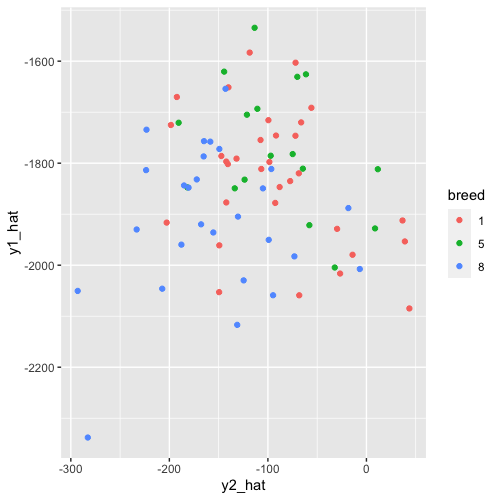
\includegraphics[width=3.0in]{8_22_S_scatter.png}
	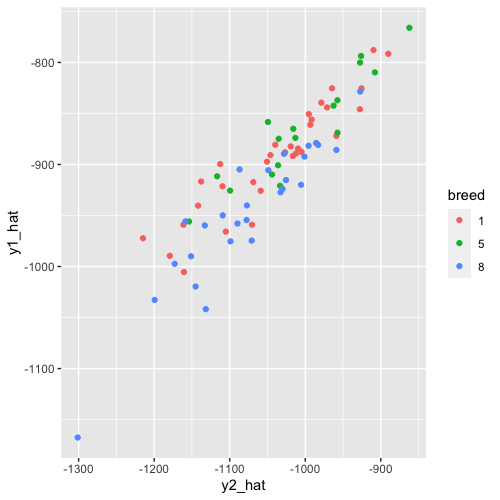
\includegraphics[width=3.0in]{8_22_R_scatter.png}
\end{center}

\item[\bf{e)}]
	A quantile-quantile plot of the data expressed via the first principal component suggests that the data is roughly normal with a large negative outlier. This holds for both the PCA on $\mf{S}$ (left) and the PCA on $\mf{R}$ (right).

\begin{center}
	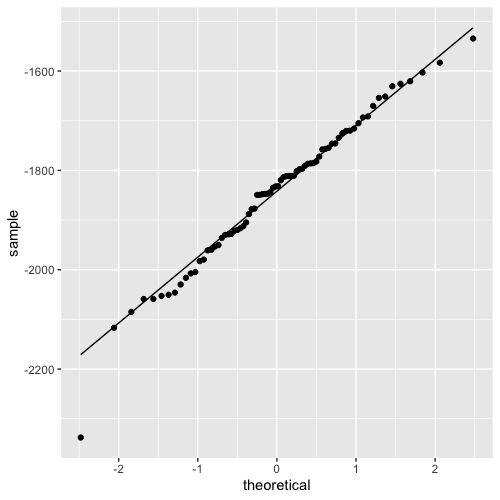
\includegraphics[width=3.0in]{8_22_S_qq.png}
	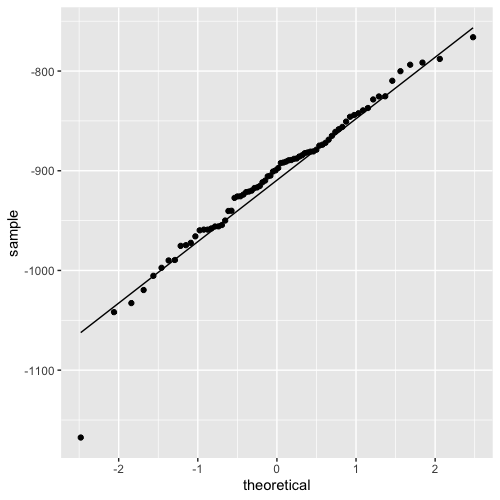
\includegraphics[width=3.0in]{8_22_R_qq.png}
\end{center}

\end{enumerate}

\end{document}
